\documentclass[a4paper, 12pt]{article}

\usepackage{amsmath}
\usepackage{amssymb}
\usepackage{graphicx}
\usepackage{xspace}
\usepackage{cleveref}
\usepackage{booktabs}
\usepackage[parfill]{parskip}



\newcommand{\pt}{\ensuremath{p_{\mathrm{T}}}\xspace}

\begin{document}

\section{Introduction}
Charged particles will bend in a magnetic field. 
For the purposes of a tracking detector, such as the one used in ATLAS, it is important to know how much a particle's trajectory will change as it traverses a tracker. 
Shown below is some of the mathematics used to calculate bending radii in certain cases, and some plots illustrating this.  

\subsection{Coordinate system}
The coordinate system is shared with the ATLAS experiment. 
The $z$ direction is along the beam pipe, the positive $y$ direction vertically upwards and the $x$ direction towards the centre of the LHC ring. 

\section{Bending radius calculation}
We consider the Lorentz force law
\begin{equation}
  \mathbf{F} = q( \mathbf{E} + \mathbf{v} \times \mathbf{B})
\end{equation}
For the ATLAS detector, the barrel tracker is cylindrical around the beam-pipe. 
The magnetic field is generated by a solenoid which surrounds the cylindrical tracker, and as a result points only in the $z$ direction, so 
$\mathbf{B} = B \mathbf{\hat{z}}$. 
There is no electric field. 
The trajectory of a charged particle will therefore only be modified in the $x$--$y$ plane, and we can therefore collapse the problem to that plane. 
To simplify further, we can assume that the initial velocity of the charged particle is along the $x$ direction, $\mathbf{v} = v \mathbf{\hat{x}}$
The Lorentz force law then collapses to
\begin{equation}
  F  = qvB
\end{equation}
With the force acting in the $y$-direction. 
This equation holds for relativistic particles, however it is important to note that the force is
\begin{equation}
  F = \frac{dp}{dt} = \gamma m \frac{dv}{dt}.
\end{equation}
The force from the magnetic field will always be acting perpendicularly to the direction of motion of the charged particle (in the $x$--$y$ plane), and so this equation will hold as time evolves. 
The motion of the particle will be a circle in the $x$--$y$ plane. 

For a relativistic particle moving in a circle, the centripetal force will be 
\begin{equation}
F = \frac{\gamma m v^2}{r}
\end{equation}
equating this with the Lorentz force law yields the bending radius
\begin{equation}
r = \frac{\gamma m v}{qB}.
\end{equation}
This is more conveniently expressed in terms of momentum (or rather, transverse momentum \pt, since we are only considering motion in the plane transverse to the beam pipe)
\begin{equation}
  \boxed{
  r = \frac{\pt}{eB}.
}
  \label{eq:bendingRadius}
\end{equation}

\subsection{Deviation}
We wish to calculate the perpendicular deviation travelled by a charged particle in a magnetic field. 
The perpendicular deviation, $l$ is the perpendicular displacement to the particle's original direction of motion. 
This is shown schematically in \cref{fig:deviation}. 
In the figure, the particle does not start at the centre of the dashed circle, but instead at the `top' of the figure, and moves in the trajectory shown by the arrow. 
The distance $d$ could be, for example, the distance between the particles origin and the first tracking layer. 

\begin{figure}
  \centering
  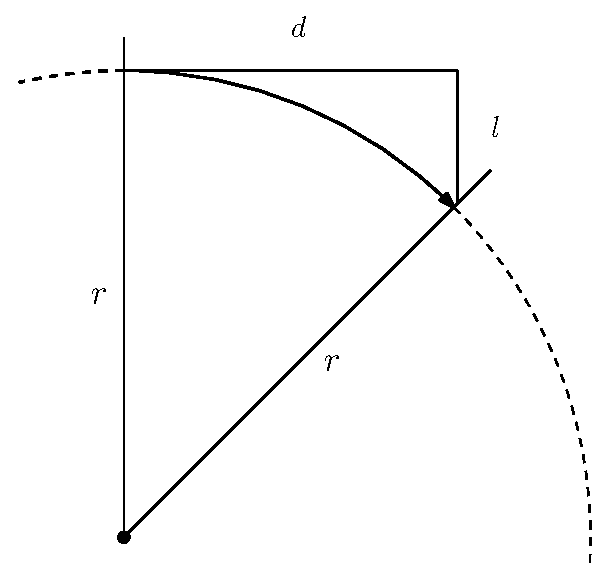
\includegraphics[width=0.5\linewidth]{images/fig1.eps}
  \caption{The deviation of a charged particle track. 
  In the absence of a magnetic field, the particle will have traversed a distance $d$.
  However, in the presence of a magnetic field, the trajectory will have deviated by a perpendicular distance $l$. 
  }
  \label{fig:deviation}
\end{figure}

One can assume that the deviation $l$ is small compared to $d$ and $r$, and is given by 
\begin{equation}
  \boxed{
  l =  r - \sqrt{r^2 - d^2}.
}
\end{equation}


\emph{Proof:} We want to find $l$ in terms of $d$ and $r$. 
The following proof is done with respect to \cref{fig:geometry}.
From Pythagoras' theorem we have 
\begin{equation}
  s^2 = l^2 + d^2.
\end{equation}
Considering the triangle within the circle, we find
$\cos \delta = (s/2)/r$
or, 
\begin{align}
  s = &\, 2r \cos \delta \\
    = &\, 2r \cos (\pi/2 - \phi) \\ 
    = &\, 2r \sin \phi. 
\end{align}
From the uppermost triangle we have $\sin \phi = l / s$, which, when combined with the above to eliminate $\sin \phi$ gives
\begin{equation}
  s^2 = 2rl.
\end{equation}
Finally, combining this with Pythagoras' theorem yields the quadratic
\begin{equation}
  l^2 - 2rl + d^2 = 0
\end{equation}
which can be solved to give
\begin{equation}
  l = r \pm \sqrt{r^2 - d^2}.
\end{equation}
We take the negative root as the correct solution as we are not interested in solutions where $l > r$ (which physically corresponds to cases where a charged particle has curled around in the magnetic
field and will miss the detector that is distance $d$ away). 


\begin{figure}
  \centering
  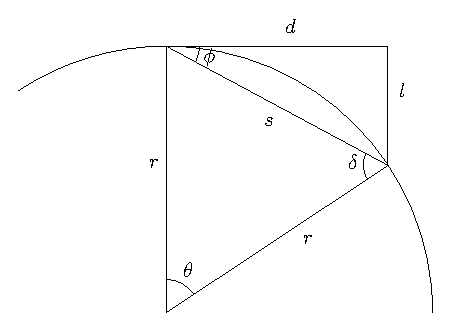
\includegraphics[width=0.4\linewidth]{images/geometry.eps}
  \caption{Geometry and definition of symbols used in the derivation of the perpendicular deviation $l$ in terms of $r$ and $d$. }
  \label{fig:geometry}
\end{figure}


\section{Useful units} 
The magnetic field of the FCC solenoid will be 4\,T. 
We wish to consider the particle momenta in GeV/c, and lengths in meters. 
Note in the following conversion from kg m s$^{-1}$ to GeV, we used the convention $[c] = c /(\mathrm{m s}^{-1})$, that is any bracketed symbol is equal to the physical constant divided by the SI
units, such that it becomes a dimensionless number  
\begin{itemize}
  \item 1 kg $\times c^2 = 9 \times 10^{16}\,\mathrm{J} = [c^2]\,\mathrm{J}$ or 1 J $ = \mathrm{kg}.c^2 / [c^2]$
  \item 1 GeV/$c = 10^9 \times 1.6 \times 10^{-19}\,\mathrm{J}/c = 10^9 \times [e] \, \mathrm{J}/c$
  \item 1 GeV/$c = 10^9 \times [e] \times 1 \, \mathrm{kg} \times c / [c^2]$
  \item 1 GeV/$c = 10^9 \times [e/c] $ kg m s$^{-1}$
  \item 1 GeV/$c = 5.344 \times 10^{-19}$ kg m s$^{-1}$
\end{itemize}
In our equation for the bending radius, we will only consider particles with charge of $1e$, therefore
\cref{eq:bendingRadius} becomes
\begin{equation}
  r\{\mathrm{m}\} = \frac{ \pt\{\mathrm{GeV}/c\} \times 10^9 \times [e/c]}{B\{\mathrm{T}\} \cdot 1\{\mathrm{C}\}[e]} 
\end{equation}
where the terms in the curly brackets are the implied units, and we have used $q = 1[e]$\,C. 
Finally, we have
\begin{equation}
  r\{\mathrm{m}\} = \frac{ \pt\{\mathrm{GeV}/c\} }{ B\{\mathrm{T}\} \cdot 1\{C\}} \times 3.35. 
\end{equation}
Further substituting in the magnetic field $B=4.0$\,T we get the quick relation
\begin{equation}
  \boxed{
  r\{m\} = 0.834 \pt \{\mathrm{GeV}/c\}.
}
  \label{eq:bendingRadiusSimp}
\end{equation}
The next question is, at what \pt will a particle bend so much that it does not reach the innermost layer of the tracker?

\section{Results}
Some quick reference numbers calculated with \cref{eq:bendingRadiusSimp} are given in \cref{tab:brquick}. 
The result of \cref{eq:bendingRadiusSimp} is also shown graphically in \cref{fig:bendingRvP}.

\begin{table}
  \centering
  \begin{tabular}{ccc}
    \toprule
    Momentum [GeV/c] & Bending radius [m] & Max deviation from origin [m] \\ 
    \midrule
    0.5 & 0.41 & 0.82 \\
    1 & 0.83   & 1.66 \\ 
    3 & 2.50   & 5.00 \\ 
    5 & 4.17   & 8.34 \\ 
    \bottomrule
  \end{tabular}
  \caption{Some quick reference numbers for bending radius for a given \pt.}
  \label{tab:brquick}
\end{table}

\begin{table}
  \centering
  \begin{tabular}{cc}
    \toprule
    Barrel layer radius [m] & Min \pt required to reach [GeV] \\ 
    \midrule 
    0.632 & 0.378 \\
    0.622 & 0.372 \\
    0.612 & 0.367 \\
    0.602 & 0.361 \\
    0.592 & 0.355 \\
    0.582 & 0.350 \\
    0.572 & 0.343 \\
    0.562 & 0.337 \\
    0.552 & 0.331 \\ 
    0.542 & 0.325 \\
    0.532 & 0.319 \\
    \bottomrule
  \end{tabular}
  \caption{Minimum \pt required to reach a barrel layer of a given radius}
\end{table}



\begin{figure}
  \centering
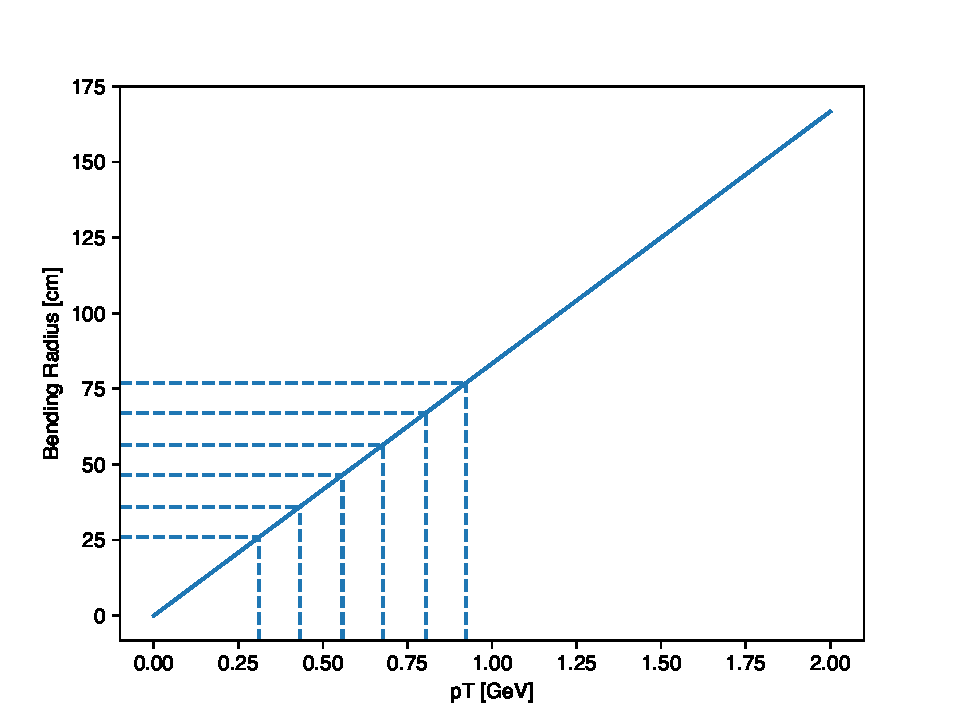
\includegraphics[width=0.5\linewidth]{images/bendingRvP}
  \caption{The bending radius of a charged particle in a magnetic field, as a function of the particle's transverse momentum. 
  The lines show approximately where different layers of the triplet would be placed. }
  \label{fig:bendingRvP}
\end{figure}











\end{document}
